%\documentclass{standalone}
%\usepackage{tikz}
%\usetikzlibrary{patterns,plotmarks}
%\begin{document}
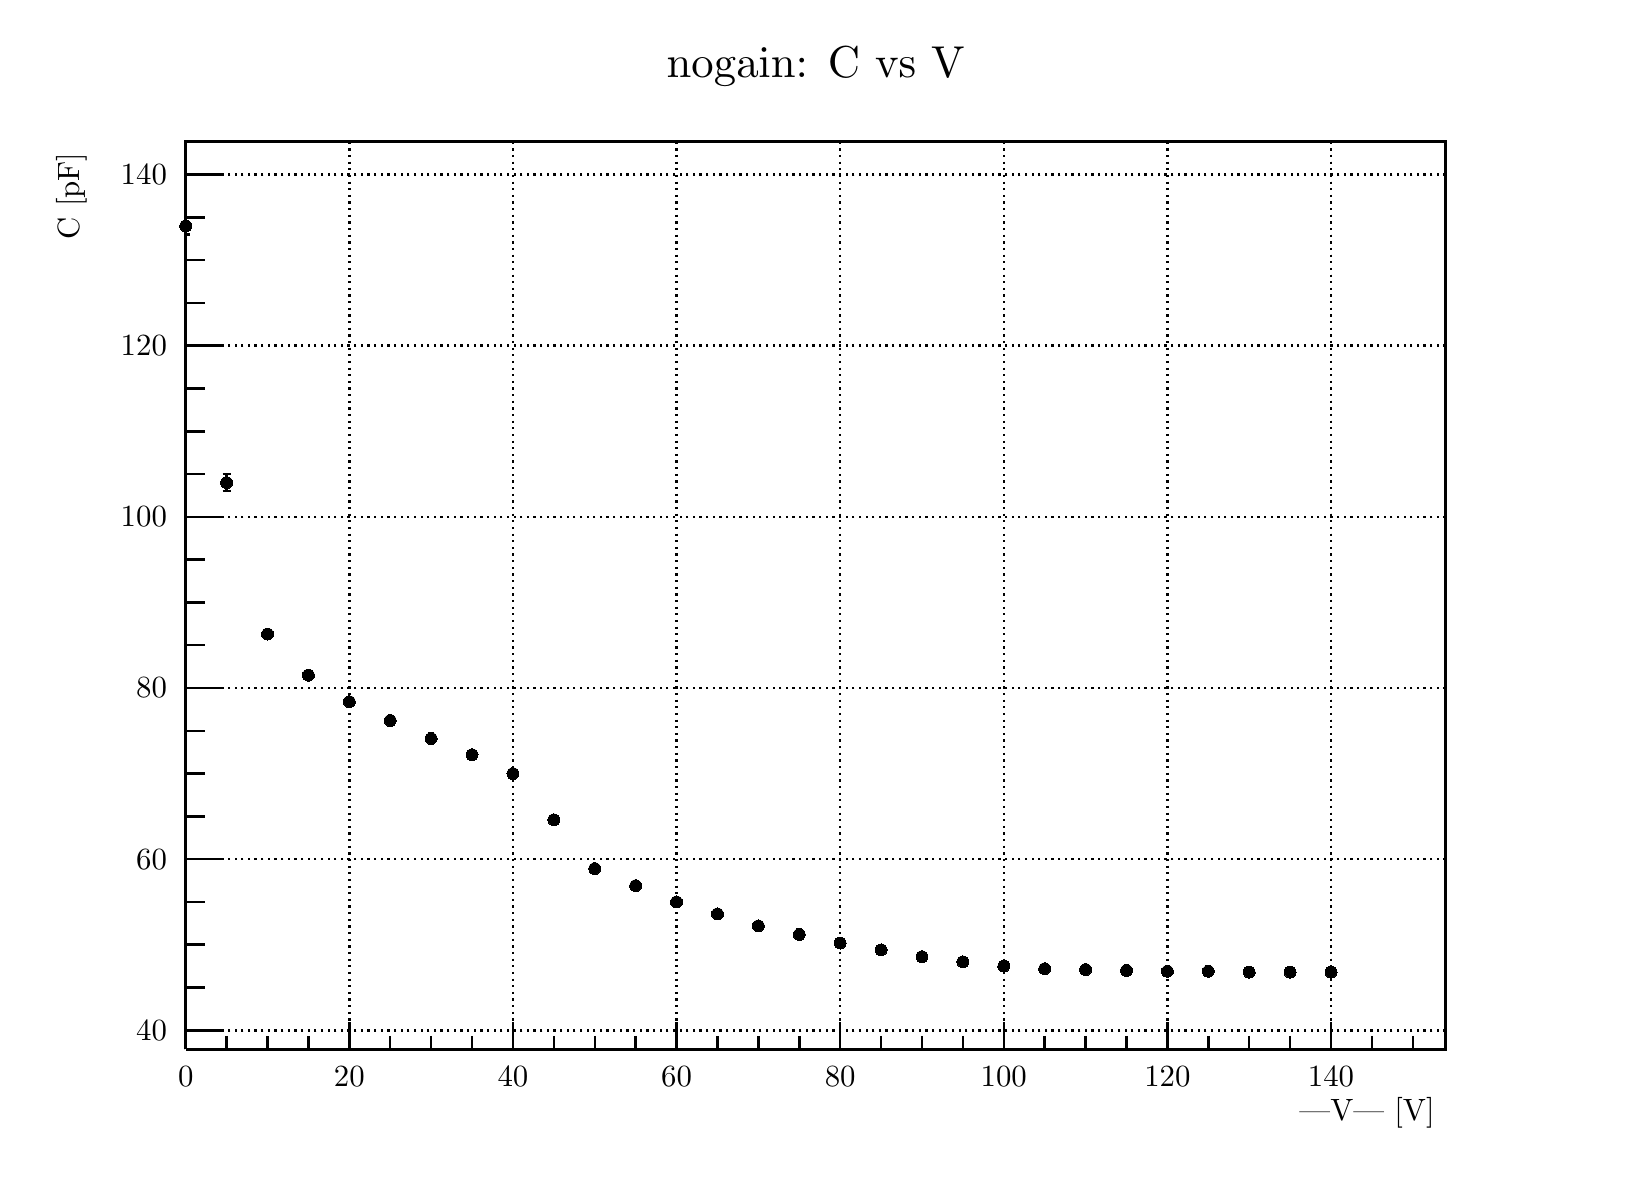
\begin{tikzpicture}
\def\CheckTikzLibraryLoaded#1{ \ifcsname tikz@library@#1@loaded\endcsname \else \PackageWarning{tikz}{usetikzlibrary{#1} is missing in the preamble.} \fi }
\CheckTikzLibraryLoaded{patterns}
\CheckTikzLibraryLoaded{plotmarks}
\pgfdeclareplotmark{cross} {
\pgfpathmoveto{\pgfpoint{-0.3\pgfplotmarksize}{\pgfplotmarksize}}
\pgfpathlineto{\pgfpoint{+0.3\pgfplotmarksize}{\pgfplotmarksize}}
\pgfpathlineto{\pgfpoint{+0.3\pgfplotmarksize}{0.3\pgfplotmarksize}}
\pgfpathlineto{\pgfpoint{+1\pgfplotmarksize}{0.3\pgfplotmarksize}}
\pgfpathlineto{\pgfpoint{+1\pgfplotmarksize}{-0.3\pgfplotmarksize}}
\pgfpathlineto{\pgfpoint{+0.3\pgfplotmarksize}{-0.3\pgfplotmarksize}}
\pgfpathlineto{\pgfpoint{+0.3\pgfplotmarksize}{-1.\pgfplotmarksize}}
\pgfpathlineto{\pgfpoint{-0.3\pgfplotmarksize}{-1.\pgfplotmarksize}}
\pgfpathlineto{\pgfpoint{-0.3\pgfplotmarksize}{-0.3\pgfplotmarksize}}
\pgfpathlineto{\pgfpoint{-1.\pgfplotmarksize}{-0.3\pgfplotmarksize}}
\pgfpathlineto{\pgfpoint{-1.\pgfplotmarksize}{0.3\pgfplotmarksize}}
\pgfpathlineto{\pgfpoint{-0.3\pgfplotmarksize}{0.3\pgfplotmarksize}}
\pgfpathclose
\pgfusepathqstroke
}
\pgfdeclareplotmark{cross*} {
\pgfpathmoveto{\pgfpoint{-0.3\pgfplotmarksize}{\pgfplotmarksize}}
\pgfpathlineto{\pgfpoint{+0.3\pgfplotmarksize}{\pgfplotmarksize}}
\pgfpathlineto{\pgfpoint{+0.3\pgfplotmarksize}{0.3\pgfplotmarksize}}
\pgfpathlineto{\pgfpoint{+1\pgfplotmarksize}{0.3\pgfplotmarksize}}
\pgfpathlineto{\pgfpoint{+1\pgfplotmarksize}{-0.3\pgfplotmarksize}}
\pgfpathlineto{\pgfpoint{+0.3\pgfplotmarksize}{-0.3\pgfplotmarksize}}
\pgfpathlineto{\pgfpoint{+0.3\pgfplotmarksize}{-1.\pgfplotmarksize}}
\pgfpathlineto{\pgfpoint{-0.3\pgfplotmarksize}{-1.\pgfplotmarksize}}
\pgfpathlineto{\pgfpoint{-0.3\pgfplotmarksize}{-0.3\pgfplotmarksize}}
\pgfpathlineto{\pgfpoint{-1.\pgfplotmarksize}{-0.3\pgfplotmarksize}}
\pgfpathlineto{\pgfpoint{-1.\pgfplotmarksize}{0.3\pgfplotmarksize}}
\pgfpathlineto{\pgfpoint{-0.3\pgfplotmarksize}{0.3\pgfplotmarksize}}
\pgfpathclose
\pgfusepathqfillstroke
}
\pgfdeclareplotmark{newstar} {
\pgfpathmoveto{\pgfqpoint{0pt}{\pgfplotmarksize}}
\pgfpathlineto{\pgfqpointpolar{44}{0.5\pgfplotmarksize}}
\pgfpathlineto{\pgfqpointpolar{18}{\pgfplotmarksize}}
\pgfpathlineto{\pgfqpointpolar{-20}{0.5\pgfplotmarksize}}
\pgfpathlineto{\pgfqpointpolar{-54}{\pgfplotmarksize}}
\pgfpathlineto{\pgfqpointpolar{-90}{0.5\pgfplotmarksize}}
\pgfpathlineto{\pgfqpointpolar{234}{\pgfplotmarksize}}
\pgfpathlineto{\pgfqpointpolar{198}{0.5\pgfplotmarksize}}
\pgfpathlineto{\pgfqpointpolar{162}{\pgfplotmarksize}}
\pgfpathlineto{\pgfqpointpolar{134}{0.5\pgfplotmarksize}}
\pgfpathclose
\pgfusepathqstroke
}
\pgfdeclareplotmark{newstar*} {
\pgfpathmoveto{\pgfqpoint{0pt}{\pgfplotmarksize}}
\pgfpathlineto{\pgfqpointpolar{44}{0.5\pgfplotmarksize}}
\pgfpathlineto{\pgfqpointpolar{18}{\pgfplotmarksize}}
\pgfpathlineto{\pgfqpointpolar{-20}{0.5\pgfplotmarksize}}
\pgfpathlineto{\pgfqpointpolar{-54}{\pgfplotmarksize}}
\pgfpathlineto{\pgfqpointpolar{-90}{0.5\pgfplotmarksize}}
\pgfpathlineto{\pgfqpointpolar{234}{\pgfplotmarksize}}
\pgfpathlineto{\pgfqpointpolar{198}{0.5\pgfplotmarksize}}
\pgfpathlineto{\pgfqpointpolar{162}{\pgfplotmarksize}}
\pgfpathlineto{\pgfqpointpolar{134}{0.5\pgfplotmarksize}}
\pgfpathclose
\pgfusepathqfillstroke
}
\definecolor{c}{rgb}{1,1,1};
\draw [color=c, fill=c] (0,0) rectangle (20,14.411);
\draw [color=c, fill=c] (2,1.4411) rectangle (18,12.9699);
\definecolor{c}{rgb}{0,0,0};
\draw [c,line width=0.9] (2,1.4411) -- (2,12.9699) -- (18,12.9699) -- (18,1.4411) -- (2,1.4411);
\definecolor{c}{rgb}{1,1,1};
\draw [color=c, fill=c] (2,1.4411) rectangle (18,12.9699);
\definecolor{c}{rgb}{0,0,0};
\draw [c,line width=0.9] (2,1.4411) -- (2,12.9699) -- (18,12.9699) -- (18,1.4411) -- (2,1.4411);
\draw [c,line width=0.9] (2,1.4411) -- (18,1.4411);
\draw [c,dash pattern=on 0.80pt off 1.60pt ,line width=0.9] (2,12.9699) -- (2,1.4411);
\draw [c,dash pattern=on 0.80pt off 1.60pt ,line width=0.9] (4.07792,12.9699) -- (4.07792,1.4411);
\draw [c,dash pattern=on 0.80pt off 1.60pt ,line width=0.9] (6.15584,12.9699) -- (6.15584,1.4411);
\draw [c,dash pattern=on 0.80pt off 1.60pt ,line width=0.9] (8.23377,12.9699) -- (8.23377,1.4411);
\draw [c,dash pattern=on 0.80pt off 1.60pt ,line width=0.9] (10.3117,12.9699) -- (10.3117,1.4411);
\draw [c,dash pattern=on 0.80pt off 1.60pt ,line width=0.9] (12.3896,12.9699) -- (12.3896,1.4411);
\draw [c,dash pattern=on 0.80pt off 1.60pt ,line width=0.9] (14.4675,12.9699) -- (14.4675,1.4411);
\draw [c,dash pattern=on 0.80pt off 1.60pt ,line width=0.9] (16.5455,12.9699) -- (16.5455,1.4411);
\draw [c,dash pattern=on 0.80pt off 1.60pt ,line width=0.9] (16.5455,12.9699) -- (16.5455,1.4411);
\draw [c,line width=0.9] (2,1.4411) -- (2,12.9699);
\draw [c,dash pattern=on 0.80pt off 1.60pt ,line width=0.9] (18,1.68455) -- (2,1.68455);
\draw [c,dash pattern=on 0.80pt off 1.60pt ,line width=0.9] (18,3.85816) -- (2,3.85816);
\draw [c,dash pattern=on 0.80pt off 1.60pt ,line width=0.9] (18,6.03176) -- (2,6.03176);
\draw [c,dash pattern=on 0.80pt off 1.60pt ,line width=0.9] (18,8.20537) -- (2,8.20537);
\draw [c,dash pattern=on 0.80pt off 1.60pt ,line width=0.9] (18,10.379) -- (2,10.379);
\draw [c,dash pattern=on 0.80pt off 1.60pt ,line width=0.9] (18,12.5526) -- (2,12.5526);
\draw [c,dash pattern=on 0.80pt off 1.60pt ,line width=0.9] (18,1.68455) -- (2,1.68455);
\draw [c,dash pattern=on 0.80pt off 1.60pt ,line width=0.9] (18,12.5526) -- (2,12.5526);
\draw [c,line width=0.9] (2,1.4411) -- (18,1.4411);
\draw [c,line width=0.9] (2,1.78697) -- (2,1.4411);
\draw [c,line width=0.9] (2.51948,1.61404) -- (2.51948,1.4411);
\draw [c,line width=0.9] (3.03896,1.61404) -- (3.03896,1.4411);
\draw [c,line width=0.9] (3.55844,1.61404) -- (3.55844,1.4411);
\draw [c,line width=0.9] (4.07792,1.78697) -- (4.07792,1.4411);
\draw [c,line width=0.9] (4.5974,1.61404) -- (4.5974,1.4411);
\draw [c,line width=0.9] (5.11688,1.61404) -- (5.11688,1.4411);
\draw [c,line width=0.9] (5.63636,1.61404) -- (5.63636,1.4411);
\draw [c,line width=0.9] (6.15584,1.78697) -- (6.15584,1.4411);
\draw [c,line width=0.9] (6.67532,1.61404) -- (6.67532,1.4411);
\draw [c,line width=0.9] (7.19481,1.61404) -- (7.19481,1.4411);
\draw [c,line width=0.9] (7.71429,1.61404) -- (7.71429,1.4411);
\draw [c,line width=0.9] (8.23377,1.78697) -- (8.23377,1.4411);
\draw [c,line width=0.9] (8.75325,1.61404) -- (8.75325,1.4411);
\draw [c,line width=0.9] (9.27273,1.61404) -- (9.27273,1.4411);
\draw [c,line width=0.9] (9.79221,1.61404) -- (9.79221,1.4411);
\draw [c,line width=0.9] (10.3117,1.78697) -- (10.3117,1.4411);
\draw [c,line width=0.9] (10.8312,1.61404) -- (10.8312,1.4411);
\draw [c,line width=0.9] (11.3506,1.61404) -- (11.3506,1.4411);
\draw [c,line width=0.9] (11.8701,1.61404) -- (11.8701,1.4411);
\draw [c,line width=0.9] (12.3896,1.78697) -- (12.3896,1.4411);
\draw [c,line width=0.9] (12.9091,1.61404) -- (12.9091,1.4411);
\draw [c,line width=0.9] (13.4286,1.61404) -- (13.4286,1.4411);
\draw [c,line width=0.9] (13.9481,1.61404) -- (13.9481,1.4411);
\draw [c,line width=0.9] (14.4675,1.78697) -- (14.4675,1.4411);
\draw [c,line width=0.9] (14.987,1.61404) -- (14.987,1.4411);
\draw [c,line width=0.9] (15.5065,1.61404) -- (15.5065,1.4411);
\draw [c,line width=0.9] (16.026,1.61404) -- (16.026,1.4411);
\draw [c,line width=0.9] (16.5455,1.78697) -- (16.5455,1.4411);
\draw [c,line width=0.9] (16.5455,1.78697) -- (16.5455,1.4411);
\draw [c,line width=0.9] (17.0649,1.61404) -- (17.0649,1.4411);
\draw [c,line width=0.9] (17.5844,1.61404) -- (17.5844,1.4411);
\draw [anchor=base] (2,0.965539) node[scale=1.11327, color=c, rotate=0]{0};
\draw [anchor=base] (4.07792,0.965539) node[scale=1.11327, color=c, rotate=0]{20};
\draw [anchor=base] (6.15584,0.965539) node[scale=1.11327, color=c, rotate=0]{40};
\draw [anchor=base] (8.23377,0.965539) node[scale=1.11327, color=c, rotate=0]{60};
\draw [anchor=base] (10.3117,0.965539) node[scale=1.11327, color=c, rotate=0]{80};
\draw [anchor=base] (12.3896,0.965539) node[scale=1.11327, color=c, rotate=0]{100};
\draw [anchor=base] (14.4675,0.965539) node[scale=1.11327, color=c, rotate=0]{120};
\draw [anchor=base] (16.5455,0.965539) node[scale=1.11327, color=c, rotate=0]{140};
\draw [anchor= east] (18,0.634085) node[scale=1.11327, color=c, rotate=0]{|V| [V]};
\draw [c,line width=0.9] (2,1.4411) -- (2,12.9699);
\draw [c,line width=0.9] (2.48,1.68455) -- (2,1.68455);
\draw [c,line width=0.9] (2.24,2.22795) -- (2,2.22795);
\draw [c,line width=0.9] (2.24,2.77135) -- (2,2.77135);
\draw [c,line width=0.9] (2.24,3.31475) -- (2,3.31475);
\draw [c,line width=0.9] (2.48,3.85816) -- (2,3.85816);
\draw [c,line width=0.9] (2.24,4.40156) -- (2,4.40156);
\draw [c,line width=0.9] (2.24,4.94496) -- (2,4.94496);
\draw [c,line width=0.9] (2.24,5.48836) -- (2,5.48836);
\draw [c,line width=0.9] (2.48,6.03176) -- (2,6.03176);
\draw [c,line width=0.9] (2.24,6.57517) -- (2,6.57517);
\draw [c,line width=0.9] (2.24,7.11857) -- (2,7.11857);
\draw [c,line width=0.9] (2.24,7.66197) -- (2,7.66197);
\draw [c,line width=0.9] (2.48,8.20537) -- (2,8.20537);
\draw [c,line width=0.9] (2.24,8.74878) -- (2,8.74878);
\draw [c,line width=0.9] (2.24,9.29218) -- (2,9.29218);
\draw [c,line width=0.9] (2.24,9.83558) -- (2,9.83558);
\draw [c,line width=0.9] (2.48,10.379) -- (2,10.379);
\draw [c,line width=0.9] (2.24,10.9224) -- (2,10.9224);
\draw [c,line width=0.9] (2.24,11.4658) -- (2,11.4658);
\draw [c,line width=0.9] (2.24,12.0092) -- (2,12.0092);
\draw [c,line width=0.9] (2.48,12.5526) -- (2,12.5526);
\draw [c,line width=0.9] (2.48,1.68455) -- (2,1.68455);
\draw [c,line width=0.9] (2.48,12.5526) -- (2,12.5526);
\draw [anchor= east] (1.9,1.68455) node[scale=1.11327, color=c, rotate=0]{40};
\draw [anchor= east] (1.9,3.85816) node[scale=1.11327, color=c, rotate=0]{60};
\draw [anchor= east] (1.9,6.03176) node[scale=1.11327, color=c, rotate=0]{80};
\draw [anchor= east] (1.9,8.20537) node[scale=1.11327, color=c, rotate=0]{100};
\draw [anchor= east] (1.9,10.379) node[scale=1.11327, color=c, rotate=0]{120};
\draw [anchor= east] (1.9,12.5526) node[scale=1.11327, color=c, rotate=0]{140};
\draw [anchor= east] (0.54812,12.9699) node[scale=1.11327, color=c, rotate=90]{C [pF]};
\foreach \P in {(2,11.9005), (2.51948,8.6401), (3.03896,6.71645), (3.55844,6.19479), (4.07792,5.85788), (4.5974,5.61878), (5.11688,5.39055), (5.63636,5.18406), (6.15584,4.94496), (6.67532,4.35809), (7.19481,3.73861), (7.71429,3.52125),
 (8.23377,3.31475), (8.75325,3.1626), (9.27273,3.01045), (9.79221,2.90177), (10.3117,2.79309), (10.8312,2.70614), (11.3506,2.6192), (11.8701,2.55399), (12.3896,2.49965), (12.9091,2.46705), (13.4286,2.45618), (13.9481,2.44531), (14.4675,2.43444),
 (14.987,2.43444), (15.5065,2.42357), (16.026,2.42357), (16.5455,2.42357)}{\draw[mark options={color=c,fill=c},mark size=2.162162pt, line width=0.000000pt, mark=*] plot coordinates {\P};}
\draw [c,line width=0.9] (2,11.9757) -- (2,12.0092);
\draw [c,line width=0.9] (2,11.8253) -- (2,11.7918);
\draw [c,line width=0.9] (2,12.0092) -- (2.05013,12.0092);
\draw [c,line width=0.9] (2,11.7918) -- (2.05013,11.7918);
\draw [c,line width=0.9] (2.51948,8.71528) -- (2.51948,8.74878);
\draw [c,line width=0.9] (2.51948,8.56491) -- (2.51948,8.53141);
\draw [c,line width=0.9] (2.46936,8.74878) -- (2.56961,8.74878);
\draw [c,line width=0.9] (2.46936,8.53141) -- (2.56961,8.53141);
\draw (10,13.9179) node[scale=1.61424, color=c, rotate=0]{nogain: C vs V};
\end{tikzpicture}
%\end{document}
